\documentclass[10pt,twocolumn,letterpaper]{article}
\usepackage[margin=0.72in,columnsep=0.25in]{geometry}
\usepackage{newtxtext,newtxmath}
\usepackage{amsmath}
\usepackage{booktabs,multirow}
\usepackage{xcolor}
\usepackage{tikz}
\usetikzlibrary{arrows.meta,positioning,fit,calc}
\usepackage[font=small,labelfont=bf,skip=3pt]{caption}
\usepackage{enumitem}
\usepackage{microtype}
\usepackage[hidelinks]{hyperref}
\usepackage{titlesec}
\titlespacing*{\section}{0pt}{6pt}{3pt}
\titlespacing*{\subsection}{0pt}{4pt}{2pt}
\titleformat{\section}{\normalfont\large\bfseries}{\thesection}{0.5em}{}
\titleformat{\subsection}{\normalfont\normalsize\bfseries}{\thesubsection}{0.5em}{}
\setlist{nosep,leftmargin=*}
\setlength{\textfloatsep}{6pt}
\setlength{\floatsep}{5pt}
\setlength{\abovedisplayskip}{3pt}\setlength{\belowdisplayskip}{3pt}
\newcommand{\tv}{\textsuperscript{\dag}}  % citation to be verified
\newcommand{\pre}{\textsuperscript{\S}}   % preliminary / small-n number
\definecolor{lang}{HTML}{E8EEF9}\definecolor{perc}{HTML}{EAF5EA}\definecolor{ocs}{HTML}{FFF4DE}\definecolor{ctrl}{HTML}{F9E8E8}

\title{\vspace{-1.2em}\Large\bfseries Confidently Wrong: Keeping Real-Time Bimanual Safety Sound\\ When VLM Priors and Perception Are Miscalibrated}
\author{\normalsize Draft for internal discussion --- bimanual YOR project (simulation study) --- 2026-10-12}
\date{\vspace{-2.2em}}

\begin{document}
\maketitle

\begin{abstract}\noindent
Vision-language models (VLMs) are increasingly asked to tell robots what is safe: which objects matter, which constraints apply,
and even physical parameters such as friction. In a real-time bimanual mobile manipulator these outputs feed a safety filter that runs
at 50--200\,Hz and enforces them as if they were true. We study what goes wrong when the priors a VLM supplies, and the perception estimates
that instantiate them, are \emph{confidently wrong}, and how to keep a hard safety filter both sound and live. We build a full
language-to-control pipeline in simulation: VLM-authored analytic set constraints, an object-centric world state whose every object carries
a calibrated uncertainty set and its provenance, and hard filters (a base shield and a feedback-linearized MPC) compiled from zonotope
geometry. We organize the sim-to-real gap into four uncertainty channels---semantic, parametric, state, and model-class---plus the
dynamics of how margins enter the filter, and report a concrete failure mechanism for each. Our central claim is a simple rule:
\emph{language may specify constraints and enlarge uncertainty sets; only calibrated evidence may shrink them}, and margins must be honest
and continuous rather than merely large. Preliminary simulation evidence: a VLM friction prior that excluded the true value would have
raised the spill budget by 20\%; uncalibrated engineering margins covered the true cup position relative to the robot 0.6\% of the time versus 96\% after
calibration; and a camera-only people channel reached 0/27 contact episodes with 27/27 task completion once margins were made
non-explosive and the robot looked before moving.
\end{abstract}

\section{Introduction}
\begin{figure*}[t]
\centering
\resizebox{\textwidth}{!}{%
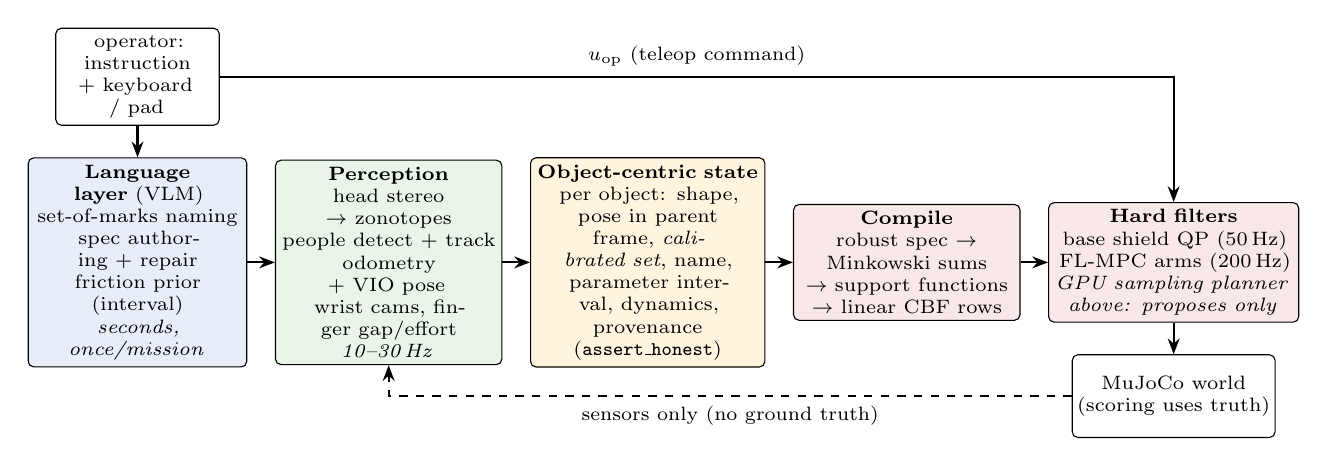
\begin{tikzpicture}[font=\scriptsize, node distance=3.5mm,
  box/.style={draw, rounded corners=2pt, align=center, minimum height=10.5mm, inner sep=2.5pt},
  arr/.style={-{Stealth[length=2mm]}, thick}]
\node[box, fill=lang, text width=26mm] (vlm) {\textbf{Language layer} (VLM)\\ set-of-marks naming\\ spec authoring + repair\\ friction prior (interval)\\ \textit{seconds, once/mission}};
\node[box, fill=perc, text width=27mm, right=of vlm] (per) {\textbf{Perception}\\ head stereo $\to$ zonotopes\\ people detect + track\\ odometry + VIO pose\\ wrist cams, finger gap/effort\\ \textit{10--30\,Hz}};
\node[box, fill=ocs, text width=28mm, right=of per] (ocs) {\textbf{Object-centric state}\\ per object: shape, pose in parent\\ frame, \emph{calibrated set}, name,\\ parameter interval, dynamics,\\ provenance (\texttt{assert\_honest})};
\node[box, fill=ctrl, text width=27mm, right=of ocs] (cmp) {\textbf{Compile}\\ robust spec $\to$ Minkowski sums\\ $\to$ support functions\\ $\to$ linear CBF rows};
\node[box, fill=ctrl, text width=30mm, right=of cmp] (flt) {\textbf{Hard filters}\\ base shield QP (50\,Hz)\\ FL-MPC arms (200\,Hz)\\ \emph{GPU sampling planner}\\ \emph{above: proposes only}};
\node[box, text width=19mm, above=4mm of vlm] (op) {operator: instruction\\ + keyboard / pad};
\node[box, text width=24mm, below=4mm of flt] (sim) {MuJoCo world\\ (scoring uses truth)};
\draw[arr] (op) -- (vlm); \draw[arr] (vlm) -- (per); \draw[arr] (per) -- (ocs); \draw[arr] (ocs) -- (cmp); \draw[arr] (cmp) -- (flt);
\draw[arr] (op.east) -- (op.east -| flt.north) node[pos=0.5,above]{$u_{\mathrm{op}}$ (teleop command)} -- (flt.north);
\draw[arr] (flt) -- (sim);
\draw[arr, dashed] (sim.west) -| node[pos=0.25,below]{sensors only (no ground truth)} (per.south);
\end{tikzpicture}}
\caption{Language-to-control pipeline. Uncertainty enters at every stage; the design question is how it propagates to the hard filter.
Ground truth is used only for scoring, and every field in the object-centric state records its source.}
\label{fig:pipe}
\vspace{-2mm}
\end{figure*}
Language is an attractive interface for safety: an operator says \emph{``bring the coffee to my desk without spilling it and keep it away
from the laptop''}, and a VLM turns that into constraints over the objects it sees. Recent work lets language models drive safety filters---an LLM infers unsafe conditions that a control-barrier filter enforces~\cite{brunke2025}, language becomes a safety specification for an MPC filter~\cite{feng2025}, or natural-language rules become verified temporal-logic monitors~\cite{safetychip}---and lets VLMs supply physical priors for sim-to-real transfer~\cite{phys2real,peng2025}.
What is rarely examined is what happens \emph{downstream}, when these outputs become the inputs of a hard real-time safety filter.
A filter is only as sound as the sets it is given: if the prior is too narrow, or the state estimate's uncertainty set does not contain
the true state, the filter certifies unsafe actions with full confidence.

Our setting makes this sharp. A holonomic base with a lift and two 6-DoF arms carries a tray holding a cup of eight loose beads through
a building under sloppy human teleoperation. The safety layer must prevent spills (contents are unobservable, so it must reason from
friction and acceleration), contact with people and furniture, and violations of the language-specified constraints, while running at
50\,Hz (base) and 200\,Hz (arms). Every quantity it uses is uncertain: the VLM's labels and parameters, the stereo geometry, the people
tracks, the robot's own pose, and the dynamics model itself.

\textbf{Problem.} \emph{What goes wrong when VLM priors and perception are miscalibrated in a real-time bimanual safety loop, and what
minimal rules keep the loop sound and live?}

\textbf{Contributions (in progress).}
(i) A language-to-control pipeline in which VLM outputs are compiled into \emph{analytic} set constraints (no learned value function in
the safety loop), evaluated on an \emph{object-centric} world state with per-object set uncertainty and provenance, so that ``fully
perception-based'' is a testable property.
(ii) A decomposition of the sim-to-real gap into four uncertainty channels plus margin dynamics, each with an observed failure mechanism
(Table~\ref{tab:uq}).
(iii) Four rules---\emph{widen-only priors}, \emph{per-object calibrated sets}, \emph{non-explosive margins}, and \emph{look before
moving}---each addressing one mechanism.
(iv) Preliminary simulation evidence for each mechanism and rule (Sec.~\ref{sec:results}). A verified search (Sec.~\ref{sec:related}) found these pieces only partially covered: no prior work measures the safety consequence of a wrong VLM \emph{physical} prior inside a hard real-time filter, states a widen-only rule, or treats margin jumps as a failure mode.

\section{Problem setting}\label{sec:setting}
\textbf{System and task.} The robot state $x$ (base pose, lift, arm joints) is controlled by an operator command $u_{\mathrm{op}}$ (base
twist, lift rate, 6-DoF tray-frame jog, grasp/release). The world contains objects $o\in\mathcal{O}$ (tray, cup, people, furniture), each
with pose $p_o$ and shape $S_o$. Physical parameters $\theta$ (here the cup--tray friction $\mu$) are unknown.

\textbf{Set-valued estimates.} Perception returns, per object, a pose estimate $\hat p_o$ and an uncertainty set
$\mathcal{U}_o=Z_o\oplus\mathcal{B}(\delta_o)$: a position zonotope $Z_o$ and a rotation-angle bound $\delta_o$. Parameters are kept as
intervals $\Theta=[\theta_{\mathrm{lo}},\theta_{\mathrm{hi}}]$. A set is \emph{calibrated at level $\alpha$} if
$\Pr[p_o\in\hat p_o\oplus\mathcal{U}_o]\ge1-\alpha$ on held-out data; we call this its \emph{coverage}.

\textbf{Specifications.} Constraints are written in a small set language: \texttt{inside}$(A,B,m)$, \texttt{upright}$(A,\vartheta)$,
\texttt{clear}$(A,B,d)$, \texttt{support}$(A,B)$, closed under $\wedge,\vee,\neg$ and the STL operators $\mathbf{G},\mathbf{F}$. Every atom has
a signed-distance robustness $\rho$~\cite{donze2010}, computed exactly on zonotopes via support functions
$h_Z(d)=c^\top d+\sum_i|g_i^\top d|$~\cite{girard2005,althoff2015}. With sets, an atom has a three-valued status:
\emph{true} if the robust margin (worst case over the sets) is $\ge0$, \emph{false} if the nominal margin is $<0$, and \emph{unknown} otherwise.
The \emph{false-safe rate} is the fraction of truly violated ticks the filter certifies as \emph{true}.

\textbf{Safety filter.} Conjunctive atoms compile to linear rows, giving
\begin{equation}
u^\star=\arg\min_u \|u-u_{\mathrm{op}}\|^2 \ \ \text{s.t.}\ \ A(\hat X,\mathcal{U},\Theta)\,u\le b(\hat X,\mathcal{U},\Theta),
\end{equation}
where the rows are high-order control-barrier conditions~\cite{ames2019} over zonotope facets, a friction-limited acceleration budget
$\|a_{\mathrm{cup}}\|\le g\min(\kappa\mu_{\mathrm{lo}},\tan\vartheta_{\mathrm{spill}})$ plus a jerk bound, and torque/clearance limits.
Soundness requires the sets to contain the truth; liveness requires them not to be so large that the program is infeasible or the robot
never moves.

\textbf{The rule.} Let $\Theta_{\mathrm{eng}}$ be a documented engineering prior and $\Theta_{\mathrm{VLM}}$ a language-model prior. We use
\begin{equation}
\Theta_{\mathrm{used}}=\begin{cases}\Theta_E, & \text{evidence }E\text{ calibrated},\\
\mathrm{hull}(\Theta_{\mathrm{eng}}\cup\Theta_{\mathrm{VLM}}), & \text{otherwise,}\end{cases}
\end{equation}
where $\Theta_E$ comes from evidence $E$ (e.g.\ a probe) with held-out coverage $\ge1-\alpha$. So a VLM can widen but never shrink the set the filter trusts. The same principle applies to state sets: they come from calibration on
residuals, not from hand-chosen $k\sigma$.

\begin{table*}[t]
\centering\small
\caption{Uncertainty channels in the pipeline: representation, calibration, and the failure observed in simulation when that channel
is left uncalibrated. \pre\,= preliminary or small $n$.}
\label{tab:uq}
\begin{tabular}{@{}p{2.6cm}p{2.9cm}p{3.3cm}p{7.3cm}@{}}
\toprule
Channel & Representation & Calibration / rule & Observed failure if uncalibrated (simulation)\\
\midrule
Semantic (names, spec) & label + confidence; spec formula & compile + semantic probes + repair; engineering fallback &
naming 54--62\% correct; self-reported confidence a constant 0.9 (uninformative); 1 of 3 specs needed repair\pre\\
Parametric (friction $\mu$) & interval $\Theta$ & \textbf{widen-only}; probes (BOED) to shrink &
VLM: $\mu\in[0.30,0.68]$ vs.\ truth 0.25 $\Rightarrow$ spill budget $1.2\times$ too permissive; planner with nominal $\mu{=}0.35$ spills 2/3 at true $\mu{=}0.18$, robust over $\Theta$ 0/3 (filter off)\pre\\
State (tray, cup, people, base, obstacles) & per-object zonotope $\oplus$ rotation bound & split conformal on residuals &
robot-frame coverage: engineering sets cup 0.006, tray 0.69 vs.\ 0.96 / 0.94 calibrated; occluded people 0.65; localizer $2\sigma$ covers $\approx$70\% after 12\,m; stereo sets hold 20--44\% of large partially-seen surfaces\\
Model class (dynamics) & per-regime residual bound & polynomial annihilation + per-regime conformal (planned) &
constant-motion cup model $\Rightarrow$ 3.55\% predictive false-safe on \texttt{inside} (18/507 ticks)\\
Margin dynamics & how a set enters the rows & non-explosive (soft-floor) margins; look before moving &
new person track with 0.5\,m margin $\Rightarrow$ infeasible program $\Rightarrow$ hard brake $\Rightarrow$ cup slides $\Rightarrow$ veto latches $\Rightarrow$ robot stuck\\
\bottomrule
\end{tabular}
\vspace{-2mm}
\end{table*}

\section{Pipeline}\label{sec:pipeline}

\textbf{Language layer.} An open VLM (Qwen3.5-9B) runs as an always-on service, at mission rate (seconds), never inside the control loop.
It (a) names perceived objects by set-of-marks prompting~\cite{som}; (b) writes the instruction as a spec in the set language, which is
compiled and checked by semantic probes (e.g.\ the spec must be violated when the container is tilted $60^\circ$), with one repair round
and a fallback to the engineering spec; and (c) elicits a friction interval in the style of Phys2Real~\cite{phys2real} (repeated queries
with self-reported $\sigma$, inverse-variance fusion).

\textbf{Perception.} Head-camera stereo gives point clouds that are segmented and fitted with order-2 hull zonotopes, inflated by the measured
depth error. People are detected from head depth and tracked with a constant-velocity Kalman filter. The base pose comes from wheel odometry
fused with a visual-inertial model (drift, latency, relocalization). The wrist cameras guide grasping, and grasp verification uses only
finger gap and gripper effort. Rendering and depth run on the GPU in separate processes (13--50$\times$ faster than CPU ray casting);
foundation stereo and model-free 6-D pose tracking~\cite{fstereo,fpose} are being added. Every model pays its start-up cost in a warm-up
phase before the robot moves.

\textbf{Object-centric state.} One \texttt{WorldState} per tick holds the robot (estimated pose and set, encoders) and every object:
shape zonotope, pose in its parent's frame (cup$\to$tray$\to$robot), a calibrated set $\mathcal{U}_o$ for the filter and a Gaussian for the
estimators, a VLM name, parameter intervals, a dynamics model (static, attached, slip-on-support, constant-velocity), and provenance
(source, measurement time, visibility, track age). Ground truth is just one producer; \texttt{privileged()} lists every ground-truth field,
so ``fully perception-based'' means the list is empty. VLM-authored specs evaluate directly on this state.

\textbf{Filters and planner.} Base rows include the friction/jerk budget, a predictive person keep-out, wall rows from a distance field,
and a zonotope clearance CBF on the base twist. Arm rows are zonotope HOCBF rows inside the feedback-linearized MPC, which also carries
arm--arm clearance, torque, and tray-tilt limits. A survey of GPU MPC methods found none with hard guarantees, so a GPU sampling planner
(MPPI~\cite{mppi}, friction sampled over $\Theta$) sits \emph{above} the filters and only proposes.

\section{Uncertainty channels and failure mechanisms}\label{sec:uq}

\textbf{Semantic.} The VLM's labels and specs are hypotheses, not facts. The model's own confidence carries no information (it was 0.9 for
every object), so acceptance cannot rest on it. Specs are accepted only if they compile and pass must-violate probes; otherwise the
engineering spec is used. Naming errors make a constraint attach to the wrong zonotope, which is why names are scored against scene metadata
and why a missing name widens, never narrows, the set of objects to keep clear of.

\textbf{Parametric.} The friction prior is the clearest instance of ``confidently wrong'': the elicited interval [0.30, 0.68] (and
[0.42, 0.81] from a second view) excluded the simulated truth 0.25. Because the spill budget scales with $\mu_{\mathrm{lo}}$, trusting the
VLM would have allowed 20\% more in-plane acceleration than the cup can tolerate. The widen-only rule removes this failure by
construction. The VLM's value is then to \emph{centre} information gathering: a Bayesian-optimal probe (BOED) can shrink $\Theta$ with
calibrated evidence. In earlier internal tests, knowing $\mu$ cut shield interventions by about 40\%. A caveat specific to simulation:
our materials are flat colours, so friction is not visually grounded, and a fair test needs textures that correlate with $\mu$.

\textbf{State.} Hand-chosen margins are both unsafe and useless. In the robot frame---the frame the cup-on-tray constraint uses---the engineering cup set contained the true cup position 0.6\% of the time (tray: 69\%),
and the certifier declared the cup constraint \emph{true} on only 2.3\% of satisfied ticks. Split-conformal sets on residuals reach
0.94--0.96 robot-frame coverage on held-out seeds. (In the world frame the same engineering sets look adequate, 0.90 and 0.999, because base-pose uncertainty dominates and hides the relative error.) For people, conformal margins give 0.927 coverage at $\alpha{=}0.05$ (0.941 uncapped), versus
0.849 for the previous $k\sigma$ margin. Two cases remain hard: occluded people (0.65 coverage; a track exists on only 46\% of occluded
ticks) and pooled calibration across episodes for the base pose, whose odometry error is a per-episode bias (pooled radius: 0.685 coverage;
we use a per-episode $k\sigma$ instead).

\textbf{Model class.} Parameter identification cannot fix a wrong model. Rolling the state forward 1\,s with a constant-twist model
missed the cup sliding after braking, giving a 3.55\% false-safe rate on the predictive \texttt{inside} atom. The conjunction stayed
unrefuted only because other atoms were \emph{unknown}. We plan to locate regime boundaries in the model residual (stick$\leftrightarrow$slip,
edge distance) with polynomial annihilation~\cite{pa}\tv{} and calibrate an error bound per regime, instead of one global bound sized for the worst case.

\textbf{Margin dynamics.} How a margin enters the filter matters as much as its size. A newly born person track arrives with a 0.5\,m
inflation, which can make the program infeasible in a single tick. The fallback brake then slides the cup, the spec monitor latches a veto
for 16--28\,s, and the robot is stuck. Capping the per-tick growth of the margin (a soft floor) and briefly yawing to look into unseen space
before moving into it remove the mechanism (Table~\ref{tab:people}).

\section{Preliminary results (simulation)}\label{sec:results}
\begin{table}[t]
\centering\small
\caption{People channel, camera-only, 9 seeds $\times$ 3 walker types (yielding, oblivious, give-up) = 27 episodes per row; new shield.
Owner-recounted from per-episode logs.}
\label{tab:people}
\begin{tabular}{@{}lcccc@{}}
\toprule
People input & contact & finished & spill & time [s]\\
\midrule
ground truth & 0 & 24 & 0 & 22.5\\
depth tracker & 3 & 11 & 3 & 28.5\\
\ + soft floor & 4 & 27 & 0 & 27.6\\
\ + conformal ($\alpha{=}.05$) & 5 & 25 & 0 & 27.9\\
\ + look before moving & 0 & 15 & 9 & 28.0\\
\ + look + soft & \textbf{0} & \textbf{27} & \textbf{0} & 30.3\\
\ + look + conformal ($\alpha{=}.20$) & \textbf{0} & \textbf{27} & \textbf{0} & 27.9\\
\bottomrule
\end{tabular}
\vspace{-1mm}
\end{table}

\textbf{People.} Table~\ref{tab:people}: neither margin fix alone nor looking alone is enough. Looking alone spills, because glances
happen while braking. Margin fixes alone still collide with side crossings outside the forward field of view. Together they reach
0 contacts and 27/27 completion, better completion than ground truth (24/27), at a cost of 5--8\,s.

\textbf{Obstacles.} With zonotopes only on the arms, the base carries the tray 106\,mm into a bottle. A zonotope clearance CBF on the base
twist kept the ball in 12/12 configurations (56\,mm true clearance, 0\,N contact force), versus 3/12 without it. It \emph{stops} rather than
going around (44\% of the path). With the GPU sampling planner proposing and the same filter certifying, the base goes around the bottle: 100\% progress, ball kept, 76\,mm clearance, 0\,N, and filter interventions on 31\% instead of 92\% of steps. With an estimated pose (4--8\,cm error), true clearance
ranged 35--78\,mm with no contacts in 9/9 seeds\pre.

\textbf{A filter-induced hazard.} Per-row (selective) slack, intended to avoid disabling all constraints when one is hopeless, flipped the
tray ($147^\circ$, 1224\,N) when the arm was released from a large accumulated tracking error. Clipping the reference and braking instead of
coasting fixed it for the 64-row configuration.

\textbf{End to end.} In a lab$\to$cafeteria$\to$desk coffee mission with the same sloppy operator, the unshielded run failed (5/8 beads
out, cup lost, person and wall contacts), while the shielded run finished with 0 beads out and 0 contacts. This run still used ground-truth
people, base pose, and walls. The camera-only replacements above are being integrated behind a single full-perception switch that must pass
\texttt{assert\_honest()}.


\section{Related work}\label{sec:related}
\textbf{Language-driven safety filters.} LLM/VLM semantics enforced by a CBF filter for manipulation~\cite{brunke2025} and dual-arm
control~\cite{gfvla}, language-conditioned MPC filters for navigation~\cite{feng2025}, verified NL$\to$LTL monitors~\cite{safetychip}, and
guardrails against adversarial prompts~\cite{roboguard} all treat the language output as correct. Closest to us, Predictive Semantic
Safety~\cite{pss} calibrates VLM \emph{event/displacement} predictions with split conformal prediction inside a 50\,Hz backup-CBF filter
(quadruped, simulation) and declines to shrink the calibrated radius from the VLM's hypothesis spread; a VLM-regulated CBF caps the VLM's
gain by geometry~\cite{alphaadj}. Neither states or tests a widen-only rule, uses physical priors, or studies wrong VLM output.
\textbf{VLM physical priors.} Phys2Real fuses a VLM centre-of-mass prior with online estimates and notes the VLM ``may be confidently
wrong''~\cite{phys2real}; overestimated VLM friction makes a locomotion policy aggressive~\cite{peng2025}; a VLM friction/mass estimate has
been checked by a CBF layer at sub-second, non-real-time rates without calibration~\cite{physician}. None measures interval coverage or the
safety cost of a wrong prior inside a hard filter. \textbf{Uncertainty in filters.} Measurement-robust CBFs~\cite{dean2020},
conformally calibrated latent safety filters~\cite{seo2025}, mismatch-adaptive shields~\cite{lu2025}, conformal safe
planning~\cite{lindemann2023}, and conformal LLM planning~\cite{knowno} each handle one uncertainty type; none combines language-sourced and
state uncertainty in one real-time filter. CBF-QP infeasibility is studied in general~\cite{xiao2023,rousseas2025,hsu2024}, but not the
chain \emph{margin jump}$\to$infeasible$\to$brake$\to$secondary hazard. Bimanual safety filtering under friction/mass uncertainty exists
without language or real-time claims~\cite{johansson2025}. Our contribution is the interaction of these channels in one real-time
bimanual loop.

\section{Falsifiable predictions and planned evaluation}
\begin{table}[t]
\centering\footnotesize
\caption{Predictions that would falsify the claims. Each compares our rule against the obvious alternative on the same missions.}
\label{tab:pred}
\begin{tabular}{@{}p{1.15cm}p{3.0cm}p{3.35cm}@{}}
\toprule
Claim & Experiment & Prediction (falsified if not)\\
\midrule
Widen-only & sim friction varied, VLM prior from materials that \emph{look} different & raw-VLM filter spills whenever $\mu_{\mathrm{lo}}^{\mathrm{VLM}}>\mu$; widen-only never does\\
Calibrated sets & conformal vs.\ $k\sigma$ vs.\ engineering sets per object & coverage $\ge1-\alpha$ \emph{and} higher certify-true rate and shorter task time\\
Non-explosive margins & soft floor / conformal on vs.\ off, with look & fewer infeasible ticks, no latch-and-stuck, contacts $\le$ baseline\\
Model-class bounds & per-regime vs.\ global residual bound & predictive false-safe $\le\alpha$ with less conservatism than a global bound\\
End to end & full-perception coffee mission (\texttt{assert\_honest}) & success and contact rates within the ground-truth run's, at bounded extra time\\
\bottomrule
\end{tabular}
\end{table}
Each claim in Sec.~\ref{sec:uq} is paired with an ablation (Table~\ref{tab:pred}). The protocol keeps the operator model, seeds, and
missions fixed, and changes only how uncertainty is represented and admitted. Ground truth is used only for scoring: spills (beads out of
the cup), true contact and clearance, and the per-tick status of the spec on true state, from which the false-safe rate follows. Sample sizes are pre-set ($\ge$9 seeds $\times$ 3 people behaviours per cell).

\section{Discussion, limitations, next steps}
\textbf{Limitations.} All results are in simulation, several with small $n$\pre. Some perception modules still interpret images with the
true camera pose (fixes in progress). The VLM friction test is not visually grounded. The grasp model uses stiffer fingers and added tray
handles. Object names in the state are still privileged until VLM naming is wired in.

\textbf{Next.} (a) Calibrate VLM physical priors across visually distinct materials and measure coverage. (b) Show a single BOED probe
shrinking $\Theta$ with calibrated coverage. (c) Per-regime model-error bounds that remove the predictive false-safe. (d) The full-perception
coffee mission, ablated: no UQ vs.\ naive UQ vs.\ ours. (e) Read the closest works in full (abstract-level verification so far) and compare against PSS~\cite{pss} on a shared task.

{\scriptsize
\begin{thebibliography}{99}\setlength{\itemsep}{0pt}\setlength{\parskip}{0pt}
\bibitem{ames2019} A.~D. Ames, S.~Coogan, M.~Egerstedt, G.~Notomista, K.~Sreenath, P.~Tabuada, ``Control barrier functions: Theory and applications,'' \emph{ECC}, 2019.
\bibitem{girard2005} A.~Girard, ``Reachability of uncertain linear systems using zonotopes,'' \emph{HSCC}, 2005.
\bibitem{althoff2015} M.~Althoff, ``An introduction to CORA 2015,'' \emph{ARCH Workshop}, 2015.
\bibitem{donze2010} A.~Donz\'e, O.~Maler, ``Robust satisfaction of temporal logic over real-valued signals,'' \emph{FORMATS}, 2010.
\bibitem{lindemann2023} L.~Lindemann, M.~Cleaveland, G.~Shim, G.~J. Pappas, ``Safe planning in dynamic environments using conformal prediction,'' \emph{IEEE RA-L}, 2023.
\bibitem{dean2020} S.~Dean, A.~J. Taylor, R.~K. Cosner, B.~Recht, A.~D. Ames, ``Guaranteeing safety of learned perception modules via measurement-robust control barrier functions,'' \emph{CoRL}, 2020.
\bibitem{mppi} G.~Williams et al., ``Information theoretic MPC for model-based reinforcement learning,'' \emph{ICRA}, 2017.
\bibitem{som} J.~Yang et al., ``Set-of-Mark prompting unleashes extraordinary visual grounding in GPT-4V,'' arXiv:2310.11441, 2023.
\bibitem{fpose} B.~Wen, W.~Yang, J.~Kautz, S.~Birchfield, ``FoundationPose: Unified 6D pose estimation and tracking of novel objects,'' \emph{CVPR}, 2024.
\bibitem{fstereo} B.~Wen et al., ``FoundationStereo: Zero-shot stereo matching,'' \emph{CVPR}, 2025.
\bibitem{brunke2025} L.~Brunke, Y.~Zhang, R.~R\"omer, J.~Naimer, N.~Staykov, S.~Zhou, A.~P. Schoellig, ``Semantically safe robot manipulation: From semantic scene understanding to motion safeguards,'' \emph{IEEE RA-L} 10(5), 2025.
\bibitem{feng2025} Z.~Feng, H.~Zhang, S.~Bansal, ``From words to safety: Language-conditioned safety filtering for robot navigation,'' arXiv:2511.05889, 2025.
\bibitem{safetychip} Z.~Yang, S.~S. Raman, A.~Shah, S.~Tellex, ``Plug in the safety chip: Enforcing constraints for LLM-driven robot agents,'' arXiv:2309.09919, 2023.
\bibitem{roboguard} Z.~Ravichandran, A.~Robey, V.~Kumar, G.~J. Pappas, H.~Hassani, ``Safety guardrails for LLM-enabled robots,'' arXiv:2503.07885, 2025.
\bibitem{gfvla} J.~Gu, W.~Cheng, L.~Gao, ``Graph-fused vision-language-action models for semantically safe dual-robot control via control barrier functions,'' engrXiv 10.31224/6733, 2026 (preprint).
\bibitem{pss} T.~Kim, S.~Fradi, Y.~Dai, M.~Ostaszewski, J.~Schmidhuber, ``Predictive semantic safety: From visual physical reasoning to safety-critical control,'' arXiv:2609.34356, 2026.
\bibitem{alphaadj} J.~Chen, R.~Chandra, ``Dynamic control barrier function regulation with vision-language models for safe, adaptive, and realtime visual navigation,'' arXiv:2603.21142, 2026.
\bibitem{phys2real} M.~Wang, S.~Tian, A.~Swann, O.~Shorinwa, J.~Wu, M.~Schwager, ``Phys2Real: Fusing VLM priors with interactive online adaptation for uncertainty-aware sim-to-real manipulation,'' \emph{ICRA}, 2026.
\bibitem{peng2025} B.~Peng, D.~Baek, Q.~Wang, J.~Ramos, ``Friction-aware safety locomotion for wheeled-legged robots using vision language models and reinforcement learning,'' \emph{Humanoids}, 2025.
\bibitem{physician} N.~Abdulsalam, ``PHYSICIAN: Verification of physical grounding in vision-language-action models,'' NeurIPS 2026 WiML poster.
\bibitem{seo2025} J.~Seo, K.~Nakamura, A.~Bajcsy, ``Uncertainty-aware latent safety filters for avoiding out-of-distribution failures,'' \emph{CoRL}, 2025.
\bibitem{lu2025} M.~Lu, J.~Gosain, L.~Sang, M.~Chen, ``Safe learning in the real world via adaptive shielding with Hamilton--Jacobi reachability,'' \emph{L4DC}, PMLR 283, 2025.
\bibitem{knowno} A.~Z. Ren et al., ``Robots that ask for help: Uncertainty alignment for large language model planners,'' \emph{CoRL}, 2023.
\bibitem{xiao2023} W.~Xiao, C.~G. Cassandras, C.~Belta, ``Learning feasibility constraints for control barrier functions,'' \emph{ECC}, 2023.
\bibitem{rousseas2025} P.~Rousseas, H.~Lee, D.~V. Dimarogonas, D.~Panagou, ``Feasibility analysis and constraint selection in optimization-based controllers,'' arXiv:2505.05502, 2025.
\bibitem{hsu2024} K.-C. Hsu, H.~Hu, J.~F. Fisac, ``The safety filter: A unified view of safety-critical control in autonomous systems,'' \emph{Annu. Rev. Control Robot. Auton. Syst.}, 2024.
\bibitem{johansson2025} A.~Johansson, D.~Lindmark, V.~Wiberg, M.~Servin, ``Safety filtering of robotic manipulation under environment uncertainty: a computational approach,'' arXiv:2509.12674, 2025.
\bibitem{pa} R.~Archibald, A.~Gelb, J.~Yoon, ``Polynomial fitting for edge detection in irregularly sampled signals and images,'' \emph{SIAM J. Numer. Anal.}, 2005.\tv
\end{thebibliography}
\vspace{-1mm}\noindent\dag\,not yet verified. Related-work entries were verified against primary pages on 2026-10-12, at abstract level for most.\par}
\end{document}
